\documentclass[12pt,a4paper]{article}
\usepackage[utf8]{inputenc}
\usepackage[T1]{fontenc}
\usepackage{amsmath}
\usepackage{textcomp}

\usepackage{geometry}
\geometry{a4paper,left=25mm,right=25mm, top=2cm, bottom=2cm} 

\usepackage{graphicx} %fuer bilder

\usepackage{verbatim}




 \usepackage{mathptmx}
 \usepackage[scaled=.90]{helvet}
 \usepackage{courier}



\usepackage{listings}
\usepackage{color}
 
\definecolor{dkgreen}{rgb}{0,0.6,0}
\definecolor{gray}{rgb}{0.5,0.5,0.5}
\definecolor{mauve}{rgb}{0.58,0,0.82}

\pagestyle{empty}
\lstset{numbers=left,language=C++}
\lstset{showstringspaces=false,
basicstyle=\ttfamily\footnotesize,
breaklines=true,
tabsize=3,
commentstyle=\color{dkgreen},      % comment style
inputencoding={ansinew},
title=\lstname %zeigt titel der datei an
}

\usepackage{pdfpages} % fuer pdfs
\usepackage{hyperref} % fuer url


%keine einrückungen bei absatz
\parindent 0pt

\begin{document}
\title{Übung 05}
\author{Reinhard Penn, Bernhard Selymes}
\date{April 2015}

\normalsize

%Beginn des Dokuments

\newcommand{\Uebung}{Coverage}
\newcommand{\srcpath}{../../src}
\newcommand{\simpath}{../../sim}

%Angabe
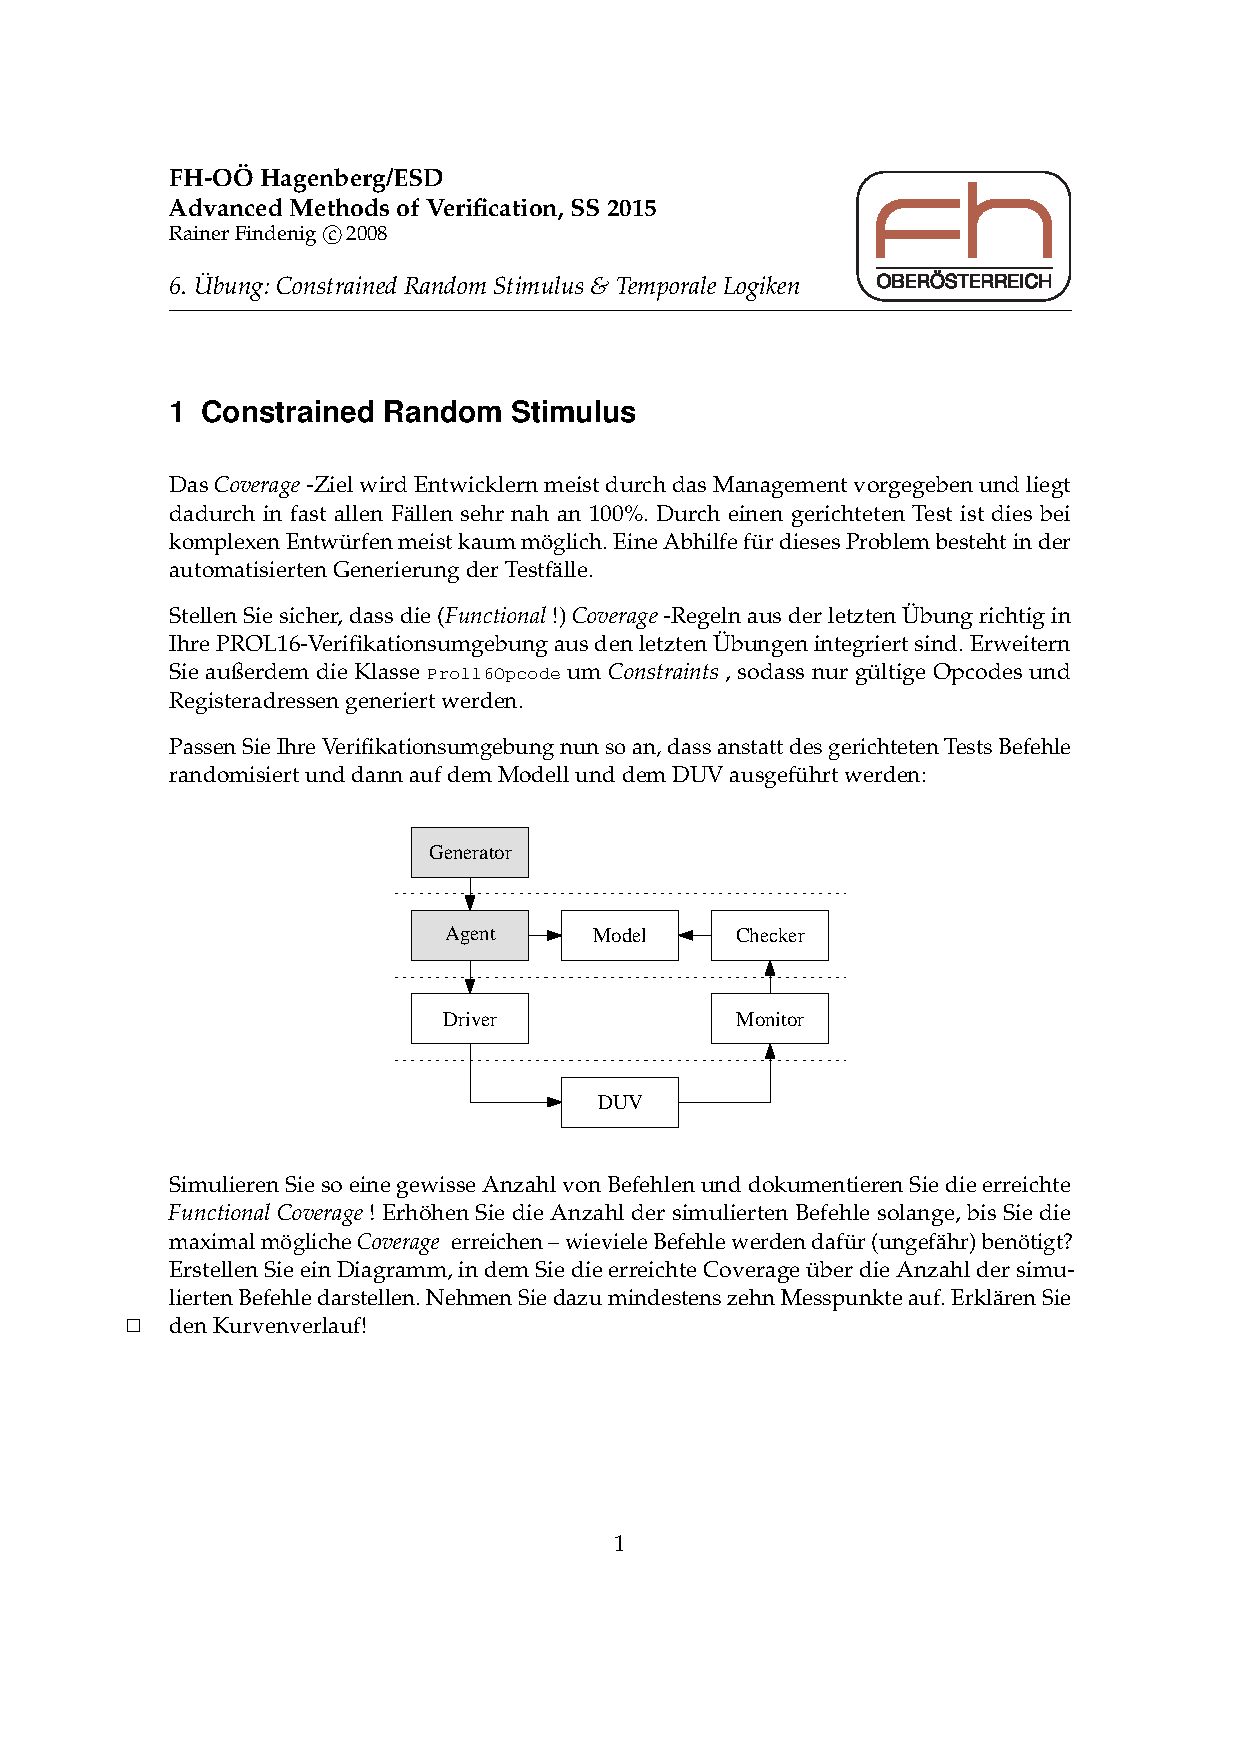
\includepdf[pages=-]{../Angabe.pdf}

\section{Beispiel 1}
\subsection{Beantwortung der Fragen}
Statement Coverage: Liefert Information darüber welche Zeilen/Statements des Codes ausgeführt wurden.

Path Coverage: Ist eine Erweiterung der Branch Coverage. Überprüft alle möglichen Kombinationen von Branches. Zum Beispiel bei zwei if-Anweisungen: true+true, false+true, true+false, false+false.

Expression Coverage: Überprüft die mögliche Werte bei einer Zuweisung und zählt mit wie oft welcher Wert zugewiesen wird. Bei einer logischen Zuweisung werden auch innere Ausdrücke betrachtet.

FSM Coverage: Gibt von einer FSM an wie oft jeder Zustand besucht wurde und wie oft jede einzele Transition ausgeführt wurde.

Hardware-Entwurf: Nein, das Problem sind z.B. die default-Zweige. Diese können dann gegebenenfalls bei der Coverage ignoriert werden.

Code Coverage: Nein, Code Coverage heißt nur, dass der Code ausgeführt wurde, aber nicht, dass er fehlerfrei ist.

\subsection{Coverage Report}

Lücken: 
\begin{itemize}
	\item Register Index = -1	-> einfach Register > 32 nehmen
	\item Register Decode Error -> siehe Register Index
	\item Falscher Opcode -> kommt darauf an ob eine falscher Opcode in das Memory geladen werden
\end{itemize}


Coverage tcl-File:
\lstinputlisting{\simpath/ComSimRegressionCoverage.tcl}

Textdatei mit Coverage Report:
\lstinputlisting{\simpath/coverage.txt}

Assemblercode:
\lstinputlisting[language={verilog}]{\simpath/regressiontest.ass}


\section{Beispiel 2}

\subsection{Source Code}

Der Sourcecode des Prol16 wurde nicht hinzugefügt, da der von der Elearning Plattform verwendet wurde.

\lstinputlisting[language={verilog}]{\srcpath/sv/ifProl16.sv}
\lstinputlisting[language={verilog}]{\srcpath/sv/pkgProl16.sv}
\lstinputlisting[language={verilog}]{\srcpath/sv/Prol16Command.sv}
\lstinputlisting[language={verilog}]{\srcpath/sv/Prol16Opcode.sv}
\lstinputlisting[language={verilog}]{\srcpath/sv/Prol16State.sv}
\lstinputlisting[language={verilog}]{\srcpath/sv/Prol16Model.sv}
%\lstinputlisting[language={verilog}]{\srcpath/sv/testProl16Model.sv}
\lstinputlisting[language={verilog}]{\srcpath/sv/testProl16Rand.sv}
\lstinputlisting[language={verilog}]{\srcpath/sv/top.sv}

\lstinputlisting[language={tcl}]{\simpath/CompileSimRandCov.do}

\end{document}
